\chapter{Descripción del compilador}

En esta parte se describe con más detalle el compilador

\section{Equipo de cómputo, lenguaje y utilerías especiales usadas en el desarrollo del proyecto}

Una PC con Windows 10, se utilizó el lenguaje de programación Python 3.10 con apoyo de las librerías de \emph{PLY, Numpy, re, json}.

Para el compilador se utilizó la librería de \emph{Ply} para el manejo del análisis léxico, sintáctico, y la semántica estática del lenguaje. En el caso del análisis semántico también se utilizó la librería de \emph{re} para manejar expresiones regulares en la lógica de semántica y código intermedio. Finalmente para poder guardar con mayor facilidad el código intermedio, la tabla de funciones y la tabla de constantes se uso la librería de JSON para exportarlos a un archivo.


\FloatBarrier
%---------------------------------------------------------------------------------------
\section{Descripción del Análisis de Léxico}

Para este lenguaje se opto por utilizar palabras clave en español. Esto se decidió con el objetivo de ser más intuitivo para las personas que hablan español y que tengan poco conocimiento del lenguaje inglés.

En IntroProg se usaron las siguientes Palabras reservadas:
\begin{itemize}
    \item programa
    \item funcion
    \item si
    \item sino
    \item mientras
    \item por
    \item entero
    \item flotante
    \item char
    \item cadena
    \item bool
    \item vacío
    \item nulo
    \item verdadero
    \item falso
    \item principal
    \item imprimir
    \item regresar
\end{itemize}

A su vez los tokens importantes del lenguaje son los siguientes:

\begin{itemize}
    \item dígito : $[0-9]$
    \item letra : $[a-zA-Z]$
    \item CTE\_INT : dígito$+$
    \item CTE\_FLOAT : dígito$+$\textbackslash .dígito$+$
    \item CTE\_STRING : \textbackslash” [ \textbackslash \textasciicircum  ” ] \textbackslash”
    \item COMMENT : \textbackslash /\textbackslash /.*
    \item espacio blanco : [ \textbackslash n\textbackslash t]$+$
    
    \item ID : letra(letra | dígito | \_ )*
    \item SEMICOLON : $;$
    \item COMMA : $,$
    \item EQ : $=$
    \item OPENPAR : \textbackslash$($
    \item CLOSEPAR : \textbackslash$)$
    \item GT : $<$
    \item LT : $>$
    \item PLUS : $+$
    \item MINUS : $-$
    \item MUL : $*$
    \item DIV : $/$
    \item OPENCUR :\textbackslash $ \{ $
    \item CLOSECUR : \textbackslash $\}$
    \item OPENSQU : \textbackslash $[$
    \item CLOSESQU : \textbackslash $]$
    \item AND : $\&\&$
    \item OR : $||$
    \item EXLAM : $!$
    \item DLR : $\$$
\end{itemize}


\FloatBarrier
%---------------------------------------------------------------------------------------
\section{Descripción del Análisis de Sintaxis}

%------------------GRAMATICA-----------------------------------------------
Con los tokens definidos en la parte léxica se desarrolló la siguiente gramática para describir el lenguaje :

{\small
\begin{enumerate}
    \item PROGRAM → PROGRAMA ID OPENCUR DECLARACIONES DECTODASFUNC PRINCIPAL FUNCION OPENCUR DECLARACIONES CLOSECUR BLOQUE CLOSECUR
    \item DECLARACIONES → DECLARACION DECLARACIONES \\ | $\epsilon$
    \item DECLARACION → DECVAR \\ \quad | DECARR
    \item DECVAR → TIPO ID DVNID SEMICOLON
    \item DVNID → COMMA ID DVNID \\ | $\epsilon$
    \item DECARR → TIPO ID OPENSQU CTE\_INT CLOSESQU DSEG SEMICOLON
    \item DSEG → OPENSQU CTE\_INT CLOSESQU DTER \\ | $\epsilon$
    \item DTER → OPENSQU CTE\_INT CLOSESQU \\ | $\epsilon$
    \item TIPO → ENTERO \\ | FLOTANTE \\ | CHAR \\ | BOOL
    \item DECTODASFUNC \\ | DECFUNC DECTODASFUNC
    \item DECFUNC →  FUNCION TIPOFUN ID OPENPAR FUNPARAM CLOSEPAR OPENCUR DECLARACIONES CLOSECUR BLOQUE
    \item TIPOFUN → TIPO \\ | VACIO
    \item FUNPARAM → PARAM \\ | $\epsilon$
    \item PARAM → TIPO ID PARAMD PARAMS
    \item PARAMS → COMMA PARAM \\ | $\epsilon$
    \item PARAMD → OPENSQU CTE\_INT CLOSESQU PDSEG \\ | $\epsilon$
    \item PDSEG → OPENSQU CTE\_INT CLOSESQU PDTER \\ | $\epsilon$
    \item PDTER → OPENSQU CTE\_INT CLOSESQU \\ | $\epsilon$
    \item BLOQUE → OPENCUR ESTATUTOS CLOSECUR
    \item ESTATUTOS → ESTATUTO ESTATUTOS \\ | $\epsilon$
    \item ESTATUTO → IMPRESION \\ | ASIGNACION \\ | EXPRESION SEMICOLON \\ | CONDICION \\ | BUCLE \\ | RETURNF
    \item IMPRESION → IMPRIMIR OPENPAR PRINTABLE PRINTARGS CLOSEPAR SEMICOLON                   
    \item PRINTARGS → COMMA PRINTABLE PRINTARGS \\ | $\epsilon$
    \item PRINTABLE → EXPRESION \\ | CTE\_STRING \\ |  $\epsilon$   
    \item ASIGNACION → ID ADIMS EQ EXPRESION  SEMICOLON \\ | ID EQ ARR\_TEX SEMICOLON
    \item ADIMS → OPENSQU EXPRESION CLOSESQU ASEGD \\ | $\epsilon$
    \item ASEGD → OPENSQU EXPRESION CLOSESQU ATERD \\ | $\epsilon$             
    \item ATERD → OPENSQU EXPRESION CLOSESQU \\ | $\epsilon$
    \item CONDICION → SI OPENPAR EXPRESION CLOSEPAR BLOQUE IFELSE
    \item IFELSE → SINO BLOQUE \\ | $\epsilon$
    \item BUCLE → WHILE \\ | FOR
    \item WHILE → MIENTRAS OPENPAR EXPRESION CLOSEPAR BLOQUE
    \item FOR → POR OPENPAR FORINIT EXPRESION SEMICOLON ASIGNACION CLOSEPAR BLOQUE
    \item FORINIT → ASIGNACION \\ | $\epsilon$
    \item RETURNF → REGRESAR EXPRESION SEMICOLON
    \item EXPRESION → EXPRESIONR \\ | EXPRLOG
    \item EXPRLOG → EXPRESION AND EXPRESION \\ | EXPRESION OR EXPRESION \\ | $\epsilon$
    \item EXPRESIONR → EXP \\ | EXPR
    \item EXPR : EXP LT EXP \\ | EXP GT EXP \\ | EXP EXLAM EQ EXP \\ | EXP EQ EQ EXP \\ | EXP LT EQ EXP \\ | EXP GT EQ EXP \\ | $\epsilon$
    \item EXP → TERMINO \\ | TERMINOSS
    \item TERMINOSS → EXP PLUS EXP \\ | EXP MINUS EXP \\ | $\epsilon$
    \item TERMINO → FACTOR \\ | FACTORESS
    \item FACTORES → TERMINO MUL TERMINO \\ | TERMINO DIV TERMINO \\ | $\epsilon$
    \item FACTOR → SIGNOVAR VARCTE \\ | OPENPAR EXPRESION CLOSEPAR
    \item SIGNOVAR → PLUS \\ | MINUS \\ | $\epsilon$
    \item VARCTE : ID \\ | CTE\_INT \\ | CTE\_FLOAT \\ | CTE\_STRING \\ | CTE\_BOOL \\ | CTE\_CHAR \\ | LLAMADAFUNC \\ | LLAMADAARR \\ | NULO
    \item LLAMADAFUNC →  DLR ID OPENPAR CALLPARAMS CLOSEPAR
    \item CALLPARAMS → CPARAM \\ | $\epsilon$
    \item CPARAM → EXPRESION CPARAMS
    \item CPARAMS → COMMA EXPRESION CPARAMS \\ | $\epsilon$
    \item LLAMADAARR → ID OPENSQU EXPRESION CLOSESQU LLSEGD
    \item LLSEGD → OPENSQU EXPRESION CLOSESQU LLTERD \\ | $\epsilon$
    \item LLTERD → OPENSQU EXPRESION CLOSESQU \\ | $\epsilon$
    \item ARR\_TEX → OPENSQU ATPRIC CLOSESQU
    \item ATPRIC → ATPRE ATPRISIG \\ | $\epsilon$
    \item ATPRE → EXPRESION \\ | ATSEGD
    \item ATPRISIG → COMMA ATPRE ATPRISIG \\ | $\epsilon$
    \item ATSEGD → OPENSQU ATSEGC CLOSESQU
    \item ATSEGC → ATSEGE ATSEGSIG \\ | $\epsilon$
    \item ATSEGE → EXPRESION \\ | ATTERD
    \item ATSEGSIG → COMMA ATSEGE ATSEGSIG \\ | $\epsilon$
    \item ATTERD → OPENSQU ATTERC CLOSESQU
    \item ATTERC → ATTERE ATTERSIG \\ | $\epsilon$
    \item ATTERE → EXPRESION
    \item ATTERSIG → COMMA ATTERE ATTERSIG \\ | $\epsilon$
    
\end{enumerate}}

Con esta gramática se procedió a generar diagramas sintácticos.


\FloatBarrier
\newpage
%---------------------------------------------------------------------------------------
\section{Descripción de Generación de Código Intermedio y Análisis Semántico}

En esta sección se explica el funcionamiento del Código Intermedio y el funcionamiento del Análisis semántico.
\subsubsection{Direcciones de Memoria Virtuales}
El compilador en todas sus operaciones asume una abstracción del manejo de memoria en la máquina virtual. Para lograr esto el compilador asigna direcciones de memoria virtuales a las constantes y variables que encuentra en su ejecución. Estas direcciones están son las siguientes.

\begin{itemize}
    \item Direcciones de las variables Globales \begin{itemize}
        \item Enteros : 1000
        \item Flotantes: 3000
        \item Caracteres :5000
        \item Booleanos: 6000
        \item Apuntadores: 7000
    \end{itemize}
    
    \item Direcciones de las Variables Locales \begin{itemize}
        \item Enteros : 9000
        \item Flotantes : 11 000
        \item Caracteres : 13 000
        \item Booleanos : 14 000
        \item Apuntadores : 15 000
    \end{itemize}
    
    \item Direcciones de las Variables Temporales \begin{itemize}
        \item Enteros: 17 000
        \item Flotantes: 19 000
        \item Caracteres: 21 000
        \item Booleanos: 22 000
        \item Apuntadores:  23 000
    \end{itemize}
    
    \item Direcciones de las Constantes \begin{itemize}
        \item Enteros: 25 000
        \item Flotantes: 27 000
        \item Caracteres: 29 000
        \item Booleanos: 30 000
        \item Cadenas:  31 000
    \end{itemize}
\end{itemize}

No solo asigna direcciones virtuales también mantiene un conteo de los recursos que se están utilizando. Si se pasa de la cantidad de variables de cada tipo y scope que se pueden usar en un espacio de memoria el compilador va a levantar un error. Estos límites son los siguientes:

\begin{itemize}
    \item Máximo de Enteros = 2000
    \item Máximo de Flotantes = 2000
    \item Máximo de Caracteres = 1000
    \item Máximo de Booleanos = 1000
    \item Máximo de Apuntadores = 2000
    \item Máximo de Cadenas = 1000
\end{itemize}

Con estos máximos se puede detectar si el usuario está declarando variables demás. Cada uno de estos máximos se dan por scope, es decir un programa puede tener un máximo de 2000 enteros globales y 2000 enteros locales en cada función. Si el usuario intenta declarar más variables que esas el compilador va a levantar un error indicando que se sobre paso el número de variables permitidos.

\subsubsection{Códigos Intermedios (Cuadruplos)}

Para el código intermedio del compilador se pensaron en las acciones básicas que debe de hacer la máquina virtual. Para indicar estas acciones se utilizaron el formato de cuádruplos para representar estos códigos. Teniendo claro esto, se definieron cuáles son las acciones más importantes que se necesitan para traducir el lenguaje a operaciones que la máquina virtual pueda interpretar con facilidad. Las acciones que son de interés para que la máquina virtual las ejecute son principalmente acciones de expresiones, asignación, saltos, manejo de memoria y código de funciones especial. Con esto en mente se desarrollaron los siguientes códigos:

\begin{itemize}
    \item \emph{Códigos de Expresiones y Asignación:} Son códigos de operación que se enfocan en realizar operaciones de expresión. Estos están formados por el operador, el cual puedes ser cualquiera de los operadores de expresiones ($+$,$-$,*, /, etc), seguidos por el operando izquierdo, seguido por el operando derecho y en la cuarta posición se la dirección virtual del resultado. Solo existe un caso especial con expresiones, el cual es cuando el operador es un $+$ o un $-$, el cual puede recibir un solo operando y este representa cuando se definen números positivos y negativos.
    
    % Ejemplos de cuadruplos de expresiones
    \begin{figure}[!htbp]
        \centering
        \begin{lstlisting}
           ["/", 17000, 25007, 17001]
           ["*", 17001, 25008, 17002]
           ["+", 25006, 17002, 17003]
           ["-", 25001, 25009, 17004]
           ["<", 17007, 25008, 22001]
           [">", 17007, 25008, 22001]
           [">=", 17007, 25008, 22001]
           ["<=", 17007, 25008, 22001]
           ["==", 17007, 25008, 22001]
           ["!=", 17007, 25008, 22001]
           ["||", 22000, 22001, 22002]
           ["&&", 22002, 30000, 22003]
           ["=", 22003, "", 14000]
        \end{lstlisting}
        \caption{Ejemplos de códigos Expresiones y asignación}
        \label{fig:my_label}
    \end{figure}
    \FloatBarrier
    
    \item \emph{Código de Saltos:} Son códigos que expresan un salto a otra instrucción. Existen dos tipos de este código los cuales son GOTO y GOTOF. El primero está conformado por la palabra clave GOTO en la primera posición y en la última posición el número del cuádruplo a donde saltar. El segundo código tiene un comportamiento diferente al primero. Este código se usa para indicar que se debe de hacer el salto si el valor en una dirección es falsa. La Composición de este cuádruplo estará dada por la palabra GOTOF en la primera posición, la dirección a evaluar en la segunda y en la última posición el número del cuádruplo a donde hacer el salto si la expresión es falsa.
    
    % Ejemplos de cuadruplos de saltos
    \begin{figure}[!htbp]
    \centering
    \begin{lstlisting}
       [ 'GOTOF' 22003 '' 112 ]
       [ 'GOTO' '' '' 91 ]
    \end{lstlisting}
    \caption{Ejemplos de códigos de saltos}
    \label{fig:my_label}
\end{figure}
\FloatBarrier
    
    \item \emph{Código de Funciones:} Son cuádruplos que indican las acciones necesarias para ejecutar funciones. Para las funciones se crear cuatro códigos para indicar su comportamiento. Estos son ERA, PARAMETER, GOTOSUB, ENDFUNC y SPFUNC. ERA es un código que indica la creación de un nuevo espacio de memoria. Este se genera escribiendo el código ERA en la primera posición y en la segunda el nombre de la función. El segundo código, PARAMETER, es un código utilizado para indicar que se debe de copiar la información de una variable a el nuevo espacio de memoria generado. Este código se escribe en un cuádruplo como la palabra clave PARAMETER en la primera posición, seguida por la dirección a copiar en la segunda posición. La tercera posición se puede dejar vacía si es una variable simple, pero si es un arreglo se escribe el tamaño en ella. Y en la última posición se escribe el tipo del parámetro y el número del parámetro separados por el símbolo \#. El tercer código es GOTOSUB. Este código sirve para indicar el cambio de contexto a una función. Este código se escribe poniendo la palabra clave GOTOSUB en la primera posición, el nombre de la función en la segunda posición. En la última posición se escribe el número del cuádruplo donde empieza la función. El cuarto código ENDFUNC sirve para indicar el fin de una función y el regreso al contexto anterior de la memoria. Este cuádruplo es muy sencillo y consta solo de la palabra clave ENDFUC en la primera posición. Finalmente se tiene el código SPFUNC. Este código se utiliza para indicar el uso de una función especial, en vez de una función del programa. Este código se genera de la siguiente manera. En la primera posición se escribe la palabra clave SPFUNC, en la segunda se escribe el nombre de la función, en la tercera posición el tipo de la función y en la última posición se escribe la dirección de la variable global de retorno si es una función que regresa un valor, sino se deja vacío.
    
    % Ejemplos de cuadruplos de funciones
\begin{figure}[!htbp]
    \centering
    \begin{lstlisting}
        ["PARAMETER", 25001, "", "1#1"]
        ["ERA", "pop", "", ""]
        ["GOTOSUB", "pop", "", 1]
        ["ENDFUNC" , "", "", ""]
        ["SPFUNC", "dexponencial", 1, 3026]
        ["SPFUNC", "diagramaDeCaja", -1, ""]
    \end{lstlisting}
    \caption{Ejemplos de códigos de funciones}
    \label{fig:my_label}
\end{figure}
\FloatBarrier
\end{itemize}

\subsubsection{Cubo Semántico}
Para el uso del código intermedio para expresiones se definio como interactuan los tipos de las variables cuando se realizan cada tipo de operación. Esto esta dado por la siguiente tabla.

\begin{table}
    \centering
    \caption{Tabla representando el cubo semántico}
    \small
    \begin{tabular}{||c c || c c c c c c c c c c c c c||} 
         
         OpIzq & OpDer & $=$ & $\parallel$ & \&\& & \textless & \textgreater & \textless $=$ & \textgreater $=$ & !$=$ & $==$ & $+$ & $-$ & * & \textbackslash \\ [0.5ex] 
         \hline\hline
         ent & ent & ent & bool & bool & bool & bool & bool & bool & bool & bool & ent & ent & ent & ent \\ 
         \hline
         ent & flot & ent & bool & bool & bool & bool & bool & bool & bool & bool & flot & flot & flot & flot \\ 
         \hline
         ent & char & ent & bool & bool & bool & bool & bool & bool & bool & bool & ent & ent & ent & ent \\ 
         \hline
         ent & bool & ent & bool & bool & bool & bool & bool & bool & bool & bool & ent & ent & ent & ent \\ 
         \hline
         ent & cadena & err & err & err & err & err & err & err & err & err & err & err & err & err \\ 
         \hline
         flot & ent & flot & bool & bool & bool & bool & bool & bool & bool & bool & flot & flot & flot & flot \\ 
         \hline
         flot & flot & flot & bool & bool & bool & bool & bool & bool & bool & bool & flot & flot & flot & flot \\ 
         \hline
         flot & char & flot & bool & bool & bool & bool & bool & bool & bool & bool & flot & flot & flot & flot \\ 
         \hline
         flot & bool & flot & bool & bool & bool & bool & bool & bool & bool & bool & flot & flot & flot & flot \\ 
         \hline
         flot & cadena & err & err & err & err & err & err & err & err & err & err & err & err & err \\ 
         \hline
         char & ent & char & bool & bool & bool & bool & bool & bool & bool & bool & ent & ent & ent & ent \\ 
         \hline
         char & flot & char & bool & bool & bool & bool & bool & bool & bool & bool & flot & flot & flot & flot \\ 
         \hline
         char & char & char & bool & bool & bool & bool & bool & bool & bool & bool & ent & ent & ent & ent \\ 
         \hline
         char & bool & char & bool & bool & bool & bool & bool & bool & bool & bool & ent & ent & ent & ent \\ 
         \hline
         char & cadena & err & err & err & err & err & err & err & err & err & err & err & err & err \\ 
         \hline
         bool & ent & bool & bool & bool & bool & bool & bool & bool & bool & bool & ent & ent & ent & ent \\ 
         \hline
         bool & flot & bool & bool & bool & bool & bool & bool & bool & bool & bool & flot & flot & flot & flot \\ 
         \hline
         bool & char & bool & bool & bool & bool & bool & bool & bool & bool & bool & ent & ent & ent & ent \\ 
         \hline
         bool & bool & bool & bool & bool & bool & bool & bool & bool & bool & bool & ent & ent & ent & ent \\ 
         \hline
         bool & cadena & err & err & err & err & err & err & err & err & err & err & err & err & err \\ 
         \hline
         cadena & ent & err & err & err & err & err & err & err & err & err & err & err & err & err \\ 
         \hline
         cadena & flot & err & err & err & err & err & err & err & err & err & err & err & err & err \\ 
         \hline
         cadena & char & err & err & err & err & err & err & err & err & err & err & err & err & err \\ 
         \hline
         cadena & bool & err & err & err & err & err & err & err & err & err & err & err & err & err \\ 
         \hline
         cadena & err & err & err & err & err & err & err & err & err & err & err & err & err & err \\ 
        
         
        
        \end{tabular}
        \begin{itemize}
            \item ent : Entero
            \item flot : Flotante
            \item err : Error
        \end{itemize}
    
\end{table}
\FloatBarrier

\subsubsection{Diagramas de Sintaxis y Acciones Semánticas}
A Continuación, se demuestran los diagramas sintácticos con sus acciones semánticas correspondientes.

\begin{enumerate}
    \begin{figure}[!htbp]
            \centering
            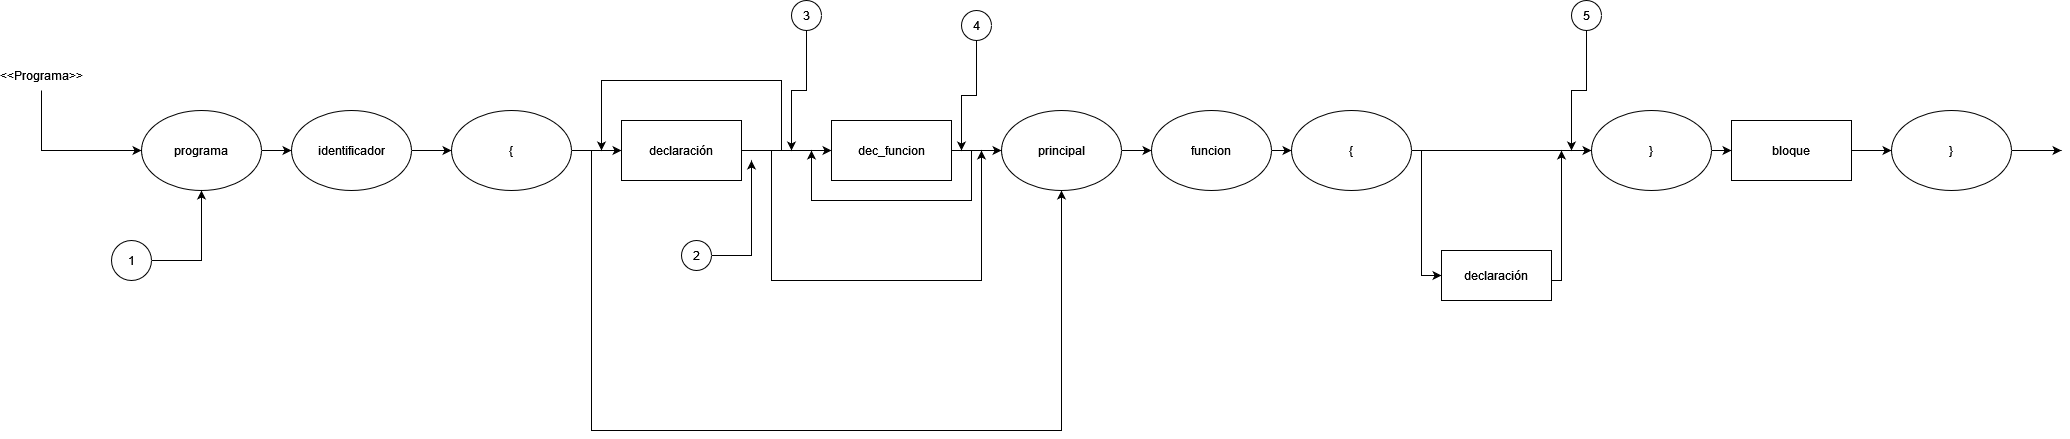
\includegraphics[width=\textwidth]{chapters/chapter3/figures/diagramas compis-Programa.drawio(1).png}
            \caption{Diagrama Programa}
            \label{fig:my_label}
    \end{figure}
    \FloatBarrier
    \item Se genera el cuádruplo de goto main y se mete el valor de contador de cuadruplos a la pila de saltos. Se actualiza la variable global del scope como global
    \item Se agrega la entrada temporal de la variable a la tabla de variables en la entrada del espacio global en el directorio de funciones.
    \item Se itera por la tabla de variables y se le asigna a cada variable una dirección virtual. Al iterar por la tabla también se actualiza el contador de recursos de las variables globales
    \item Se agrega la función a el directorio de variables
    \item Se genera la tabla de variables para el scope principal y se itera por la tabla asignando las direcciones virtuales adecuadas. Al terminar se hace pop a la pila de saltos y se actualiza el primer cuádruplo con el contador actual de cuádruplos.
    \newpage
    
    %Dec
    \begin{figure}[!htbp]
            \centering
            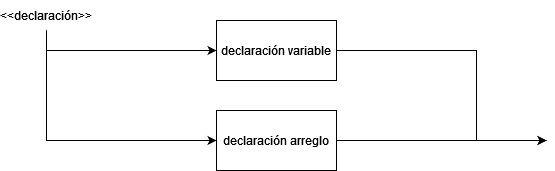
\includegraphics[width=\textwidth]{chapters/chapter3/figures/diagramas compis-declaración.drawio(1).png}
            \caption{Diagrama Declaración}
            \label{fig:my_label}
    \end{figure}
    \FloatBarrier
    % Tipo
    \begin{figure}[!htbp]
            \centering
            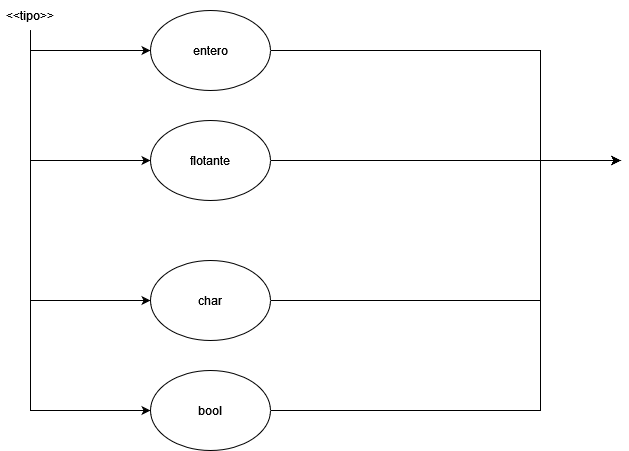
\includegraphics[width=\textwidth]{chapters/chapter3/figures/diagramas compis-tipo.drawio.png}
            \caption{Diagrama Tipo}
            \label{fig:my_label}
    \end{figure}
    \FloatBarrier
    
    %Dec de variable
    \begin{figure}[!htbp]
            \centering
            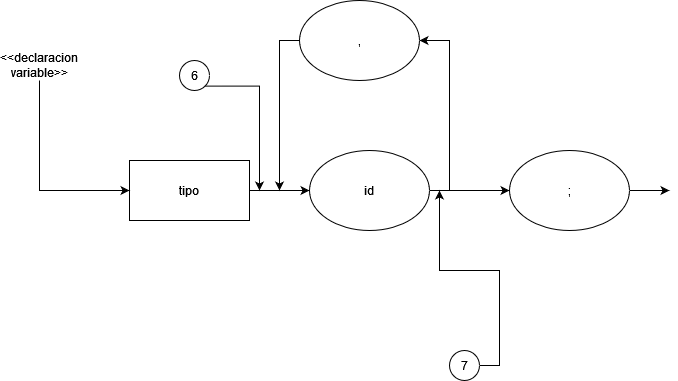
\includegraphics[width=\textwidth]{chapters/chapter3/figures/diagramas compis-declaración variable.drawio(1).png}
            \caption{Diagrama Declaración Variable}
            \label{fig:my_label}
    \end{figure}
    \FloatBarrier
    
    \item Se guarda en una variable auxiliar global el tipo de variable
    \item Se checa que el id no se repita con otros ids del scope de la declaración. Si no se repite se genera una nueva entrada de variable con el nuevo id con el tipo de variable dado por el punto 6
    
    \newpage
    %DEc de arreglo
    
    \begin{figure}[!htbp]
            \centering
            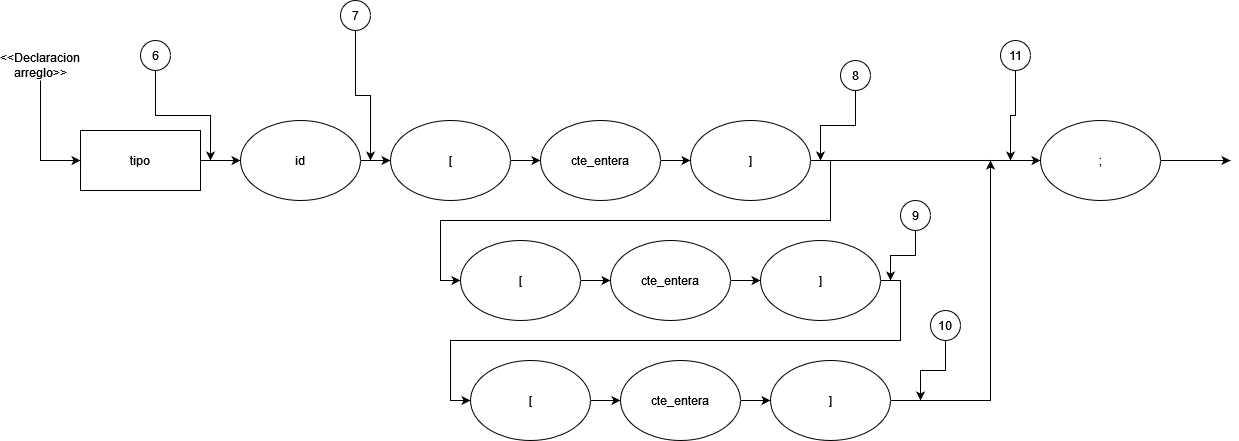
\includegraphics[width=\textwidth]{chapters/chapter3/figures/diagramas compis-declaración arreglo.drawio(1).png}
            \caption{Diagrama Declaración Arreglo}
            \label{fig:my_label}
    \end{figure}
    \FloatBarrier
    
    \item Se agrega la información de la primera dimensión a la entrada de la variable
    \item Se agrega la información de la segunda dimensión a la entrada de la variable
    \item Se agrega la información de la tercera dimensión a la entrada de la variable
    \item Se hace el cálculo de las m y el tamaño del arreglo/matriz/cubo (depende de las dimensiones leídas) y se actualiza la entrada
    
    \newpage
    % Dec Func
    
    \begin{figure}[!htbp]
            \centering
            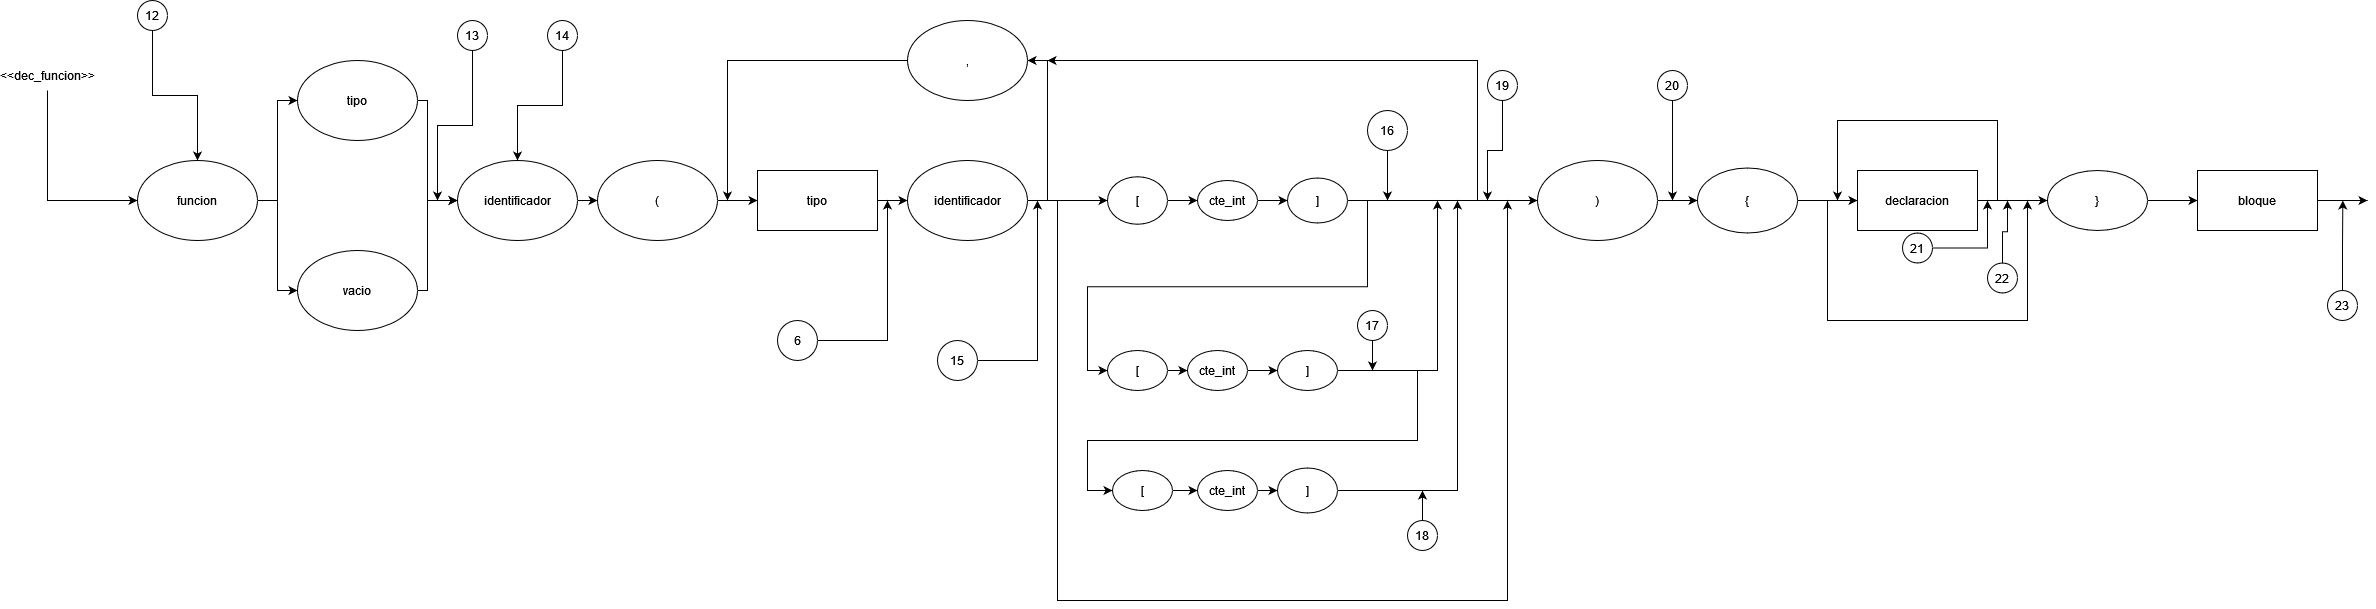
\includegraphics[width=\textwidth]{chapters/chapter3/figures/diagramas compis-dec_funcion.drawio(1).png}
            \caption{Diagrama Declaración Función}
            \label{fig:my_label}
    \end{figure}
    \FloatBarrier
    
    
    \item Se guarda en una variable auxiliar global el número del cuádruplo donde empieza la función y se genera una entrada temporal al directorio de funciones.
    \item Se guarda el tipo de función a la entrada temporal
    \item Se comprueba que el identificador no sea igual a otros identificadores, palabras clave o nombres de funciones especiales. Si no hay conflictos se agrega el nombre a la entrada temporal, si el tipo no es vacío, genera una variable global con el nombre y tipo de la función con la dirección virtual apropiada y se actualiza la variable global de scope y los contadores de recursos globales.
    \item Se checa que el id no se repita entre otros parámetros. Si no se repite se agrega el parámetro con el id y el tipo detectado a la sección de parámetros de la entrada temporal
    \item Se agrega la información de la primera dimensión a la entrada del parámetro
    \item Se agrega la información de la segunda dimensión a la entrada del parámetro
    \item Se agrega la información de la tercera dimensión a la entrada del parámetro
    \item Se hace el cálculo de las m y el tamaño del arreglo/matriz/cubo (depende de las dimensiones leídas)y se actualiza la entrada
    \item Se crean entradas a la tabla de variables locales de la funciones con la información de los parámetros
    \item Se agrega la entrada temporal de la tabla de variables a la tabla de variables local.
    \item Se itera por la tabla de variables y se le asigna a cada variable una dirección virtual.
    \item Se genera el cuádruplo de ENDFUNC y se agregan la cantidad de recursos utilizados por la función a la entrada de la función.
    
    \newpage
    
    %Bloque
    
    \begin{figure}[!htbp]
            \centering
            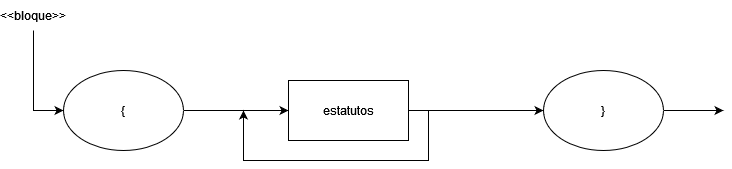
\includegraphics[width=\textwidth]{chapters/chapter3/figures/diagramas compis-bloque.drawio(1).png}
            \caption{Diagrama Bloque}
            \label{fig:my_label}
    \end{figure}
    \FloatBarrier
    
    %Estatuto
    \begin{figure}[!htbp]
            \centering
            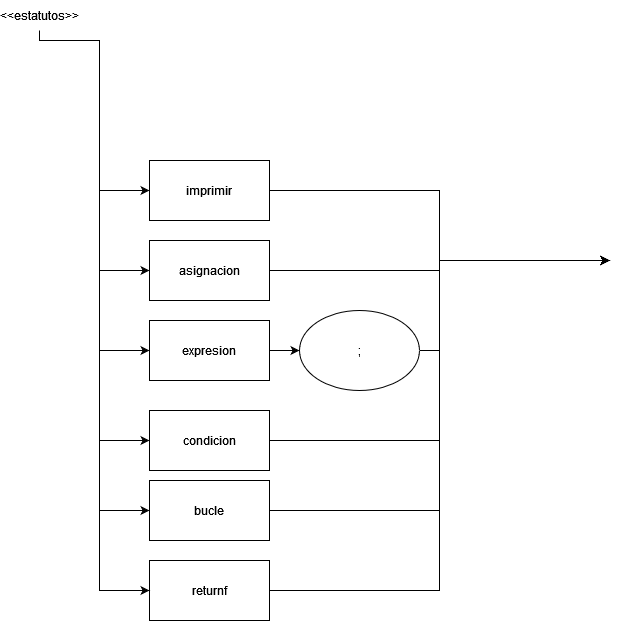
\includegraphics[width=\textwidth]{chapters/chapter3/figures/diagramas compis-estatuto.drawio(1).png}
            \caption{Diagrama Estatutos}
            \label{fig:my_label}
    \end{figure}
    \FloatBarrier
    %Return
    \begin{figure}[!htbp]
            \centering
            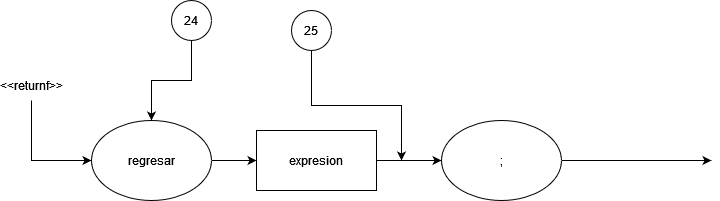
\includegraphics[width=\textwidth]{chapters/chapter3/figures/diagramas compis-returnf.drawio.png}
            \caption{Diagrama Return}
            \label{fig:my_label}
    \end{figure}
    \FloatBarrier
    \item Checar si la función que llamo a regresar no sea una función vacía. Si es vacia levantar un error
    \item Generar el cuádruplo de [RET, Dirección del resultado de la expresión, , Dirección de la variable global]
    
    \newpage
    
    %Condición
    \begin{figure}[!htbp]
            \centering
            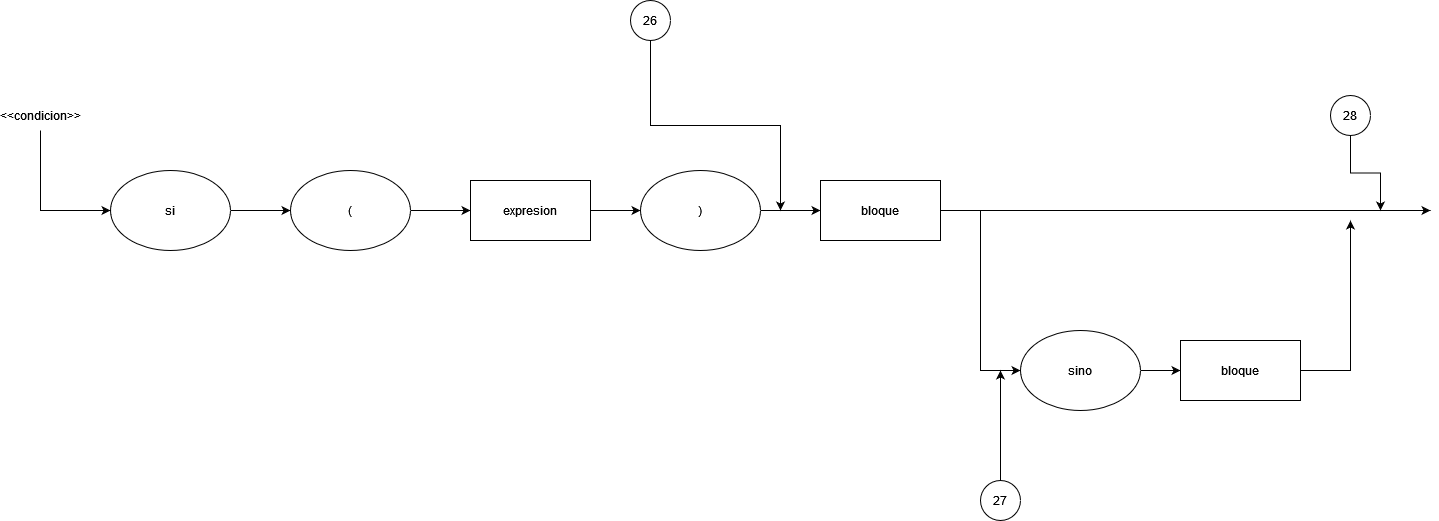
\includegraphics[width=\textwidth]{chapters/chapter3/figures/diagramas compis-condicion.drawio(1).png}
            \caption{Diagrama Condición}
            \label{fig:my_label}
    \end{figure}
    \FloatBarrier
    
    \item Se genera el cuádruplo de gotof con el resultado de la expresión y se agrega número del cuádruplo generado a la pila de saltos.
    \item Se hace pop a la pila de saltos y se genera un cuádruplo de goto y se agrega su número de cuádruplo a la pila. Se actualiza el gotof con el contador actual de cuádruplos
    \item Se hace pop a la pila de saltos y se actualiza el cuádruplo indicado por la pila con el contador actual.
    
    \newpage
    
    %Bucle
    
    \begin{figure}[!htbp]
            \centering
            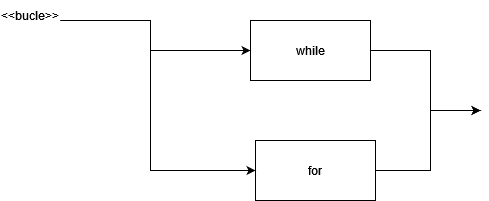
\includegraphics[width=\textwidth]{chapters/chapter3/figures/diagramas compis-bucle.drawio(1).png}
            \caption{Diagrama Bucle}
            \label{fig:my_label}
    \end{figure}
    \FloatBarrier
    
    %While
    \begin{figure}[!htbp]
            \centering
            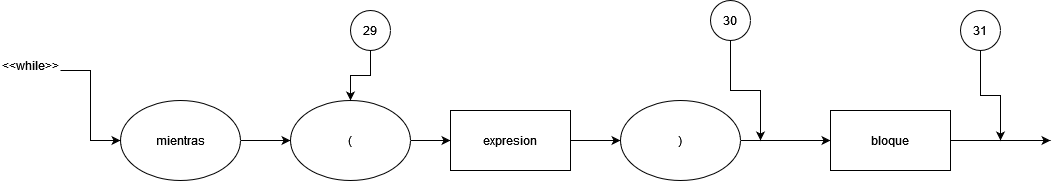
\includegraphics[width=\textwidth]{chapters/chapter3/figures/diagramas compis-while.drawio(1).png}
            \caption{Diagrama While}
            \label{fig:my_label}
    \end{figure}
    \FloatBarrier
    
    \item Se mete el contador actual de cuádruplos a la pila de operandos
    \item Se genera un cuádruplo de gotof con el resultado de la expresión y se agrega su número de contador a la pila de saltos
    \item Se le da pop dos veces a la pila de saltos y se genera un cuádruplo de goto con el segundo valor obtenido. Con el primer valor se obtiene el cuádruplo en donde esta el gotof y se actualiza con el contador actual de cuádruplos.
    
    \newpage
    %For
    \begin{figure}[!htbp]
            \centering
            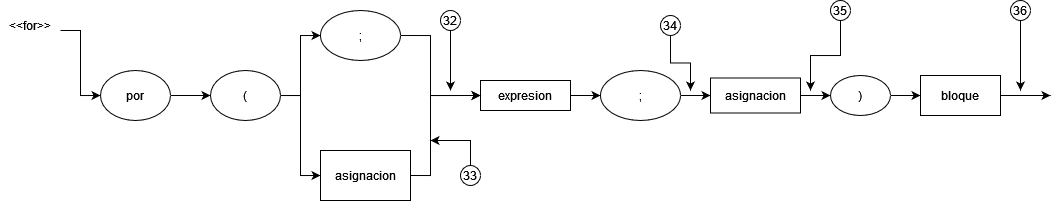
\includegraphics[width=\textwidth]{chapters/chapter3/figures/diagramas compis-for.drawio(1).png}
            \caption{Diagrama For}
            \label{fig:my_label}
    \end{figure}
    \FloatBarrier
    
    \item Se agrega el contador actual a la pila de saltos.
    \item Se checa que la asignación sea una asignación entera
    \item Se genera un gotof con la expresión y se agrega el número de cuádruplo del gotof a la pila de saltos. También se genera un cuádruplo de goto y también se agrega su número de cuádruplo a la pila de saltos.
    \item Se le hace pop a los primeros cuatro elementos de la pila de saltos. Se genera un goto al cuádruplo donde inicia la condición del for, se actualiza el cuádruplo del goto que va al bloque después de la evaluación y se vuelven a insertar los elementos sobrantes.
    \item Se le hace pop a dos elementos de la pila de operandos. Se genera un cuádruplo de goto a donde empieza la asignación de paso del for y se actualiza el cuádruplo de gotof de la condición del for.
    
    \newpage
    
    %Imprimir
    \begin{figure}[!htbp]
            \centering
            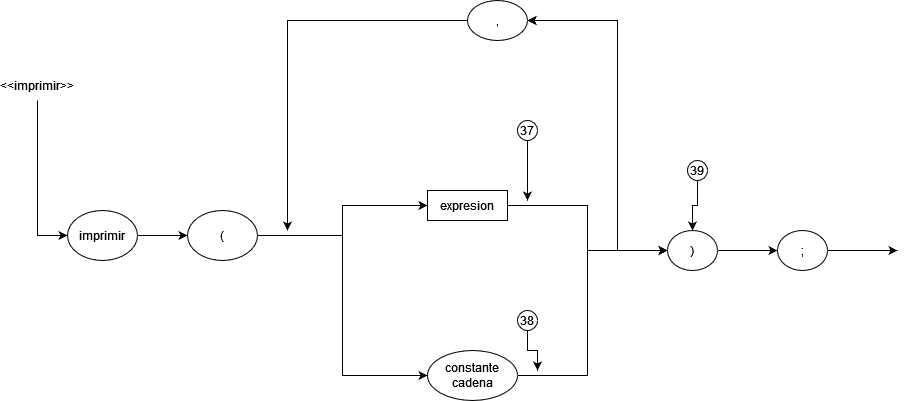
\includegraphics[width=\textwidth]{chapters/chapter3/figures/diagramas compis-imprimir.drawio(1).png}
            \caption{Diagrama Imprimir}
            \label{fig:my_label}
    \end{figure}
    \FloatBarrier
    
    \item Se le hace pop a la pila de operandos y se agrega a la fila de impresiones
    \item Se checa que la constante esta en la tabla de constantes, si no esta se agrega asignando la dirección virtual apropiada. Se agrega la dirección virtual a la pila de impresión.
    \item Se recorre la fila de impresión y se va generando un cuádruplo de imprimir con la dirección virtual en la fila
    
    \newpage
    
    %Asignación
    \begin{figure}[!htbp]
            \centering
            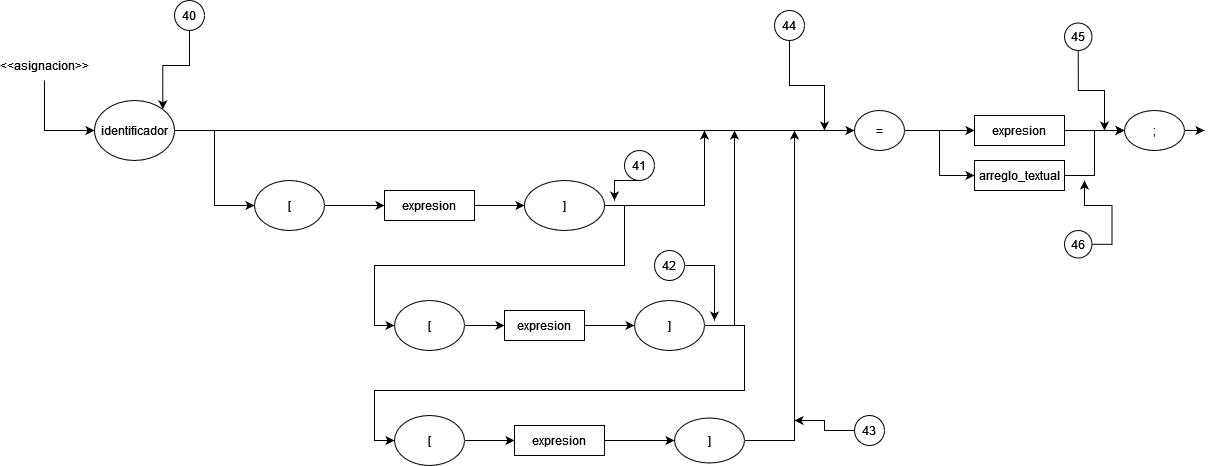
\includegraphics[width=\textwidth]{chapters/chapter3/figures/diagramas compis-asignacion.drawio(1).png}
            \caption{Diagrama Asignación}
            \label{fig:my_label}
    \end{figure}
    \FloatBarrier
    
    \item Se checa que el identificador exista en el scope local o en scope global
    \item Se hace pop a la pila de operandos y se revisa que el elemento recibido sea entero. Si es entero se agrega a la fila de subíndices.
    \item Se hace pop a la pila de operandos y se revisa que el elemento recibido sea entero. Si es entero se agrega a la fila de subíndices.
    \item Se hace pop a la pila de operandos y se revisa que el elemento recibido sea entero. Si es entero se agrega a la fila de subíndices.
    \item Se revisa si el identificador es un arreglo. Si es un arreglo se checa que la cantidad de subíndices leídos coincida con las dimensiones del arreglo, de ser así itera por los subíndices generando los cuádruplos de verificación y las sumas apropiadas para calcular la dirección virtual del arreglo accesado.
    \item Se checa contra el cubo semántico si se puede hacer la asignación. De ser posible se genera el cuádruplo de asignación apropiado.
    \item Se checa que el identificador no sea una variable simple o una llamada de arreglo. También se checa que las dimensiones del arreglo textual son iguales a las del identificador.
    
    \newpage
    
    %Expresion
    \begin{figure}[!htbp]
            \centering
            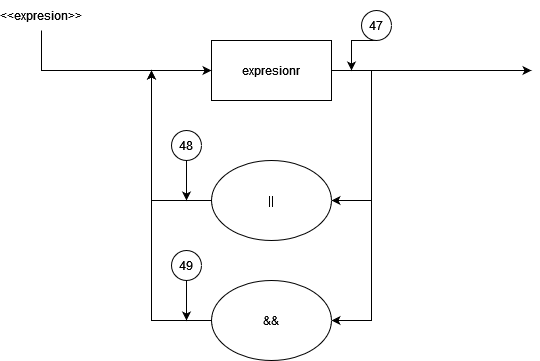
\includegraphics[width=\textwidth]{chapters/chapter3/figures/diagramas compis-expresion.drawio(1).png}
            \caption{Diagrama Expresión}
            \label{fig:my_label}
    \end{figure}
    \FloatBarrier
    
    \item Si la cima de la pila de operandos es igual a \&\& o $\parallel$, hacer pop a la pila de operandos y generar el cuádruplo de expresión correspondiente a la operador detectado.
    \item Meter $\parallel$ a la pila de operandos
    \item Meter \&\& a la pila de operandos
    
    \newpage
    
    %ExpresionR
    
    \begin{figure}[!htbp]
            \centering
            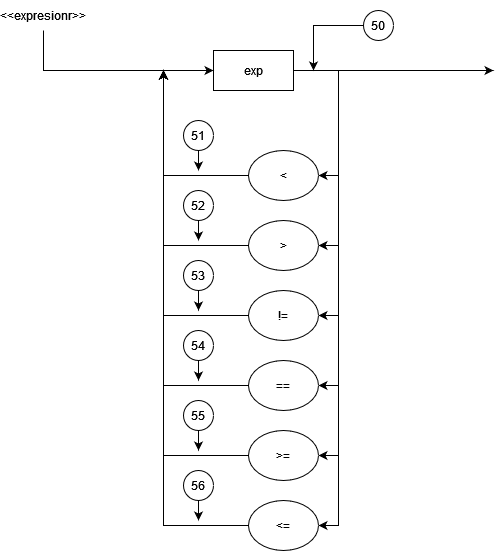
\includegraphics[width=\textwidth]{chapters/chapter3/figures/diagramas compis-expresionr.drawio.png}
            \caption{Diagrama ExpresiónR}
            \label{fig:my_label}
    \end{figure}
    \FloatBarrier
    
    \item Si la cima de la pila de operandos es igual a <, >, !=, <=, >= ó ==, hacer pop a la pila de operandos y generar el cuádruplo de expresión correspondiente a la operador detectado.
    \item Meter < a la pila de operandos
    \item Meter > a la pila de operandos
    \item Meter != a la pila de operandos
    \item Meter == a la pila de operandos
    \item Meter >= a la pila de operandos
    \item Meter <= a la pila de operandos
    \newpage
    
    %EXP
    \begin{figure}[!htbp]
            \centering
            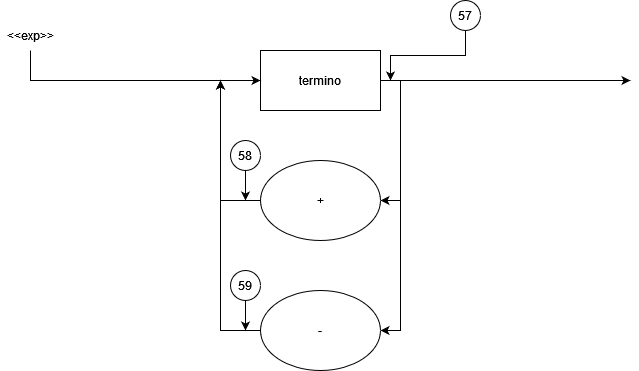
\includegraphics[width=\textwidth]{chapters/chapter3/figures/diagramas compis-exp.drawio(1).png}
            \caption{Diagrama EXP}
            \label{fig:my_label}
    \end{figure}
    \FloatBarrier
    
    \item Si la cima de la pila de operandos es igual a + ó -, hacer pop a la pila de operandos y generar el cuádruplo de expresión correspondiente a la operador detectado.
    \item Meter + a la pila de operandos
    \item Meter - a la pila de operandos
    \newpage
    
    %Termino
    \begin{figure}[!htbp]
            \centering
            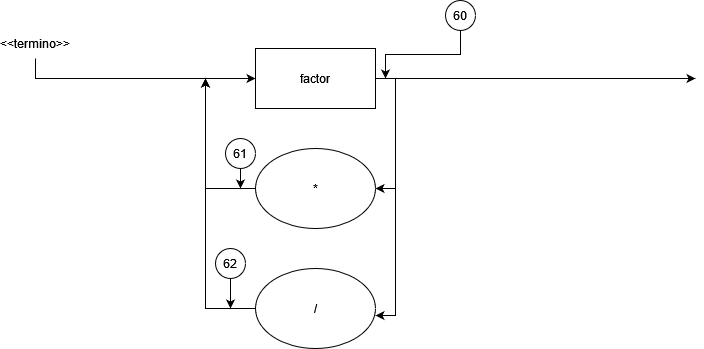
\includegraphics[width=\textwidth]{chapters/chapter3/figures/diagramas compis-termino.drawio(1).png}
            \caption{Diagrama Termino}
            \label{fig:my_label}
    \end{figure}
    \FloatBarrier
    \item Si la cima de la pila de operandos es igual a * ó /, hacer pop a la pila de operandos y generar el cuádruplo de expresión correspondiente a la operador detectado.
    \item Meter * a la pila de operandos
    \item Meter / a la pila de operandos
    \newpage
    
    %Factor
    \begin{figure}[!htbp]
            \centering
            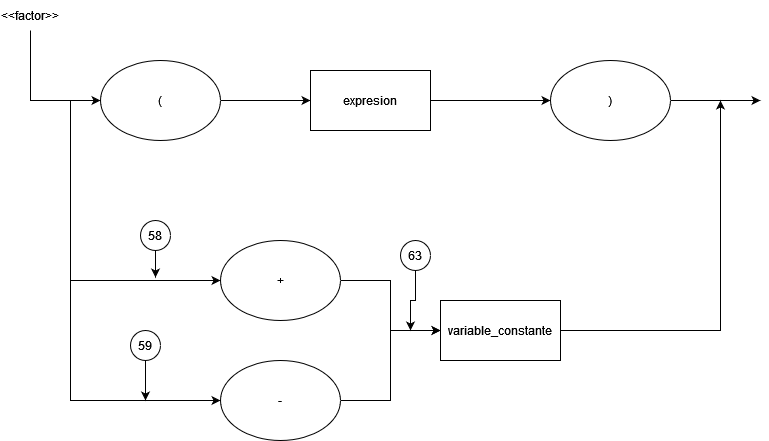
\includegraphics[width=\textwidth]{chapters/chapter3/figures/diagramas compis-factor.drawio(1).png}
            \caption{Diagrama Factor}
            \label{fig:my_label}
    \end{figure}
    \FloatBarrier
    \item Hacer pop a la pila de operador y hacer el cuádruplo de expresión unaria del operador obtenido de la pila
    
    
    \newpage
    
    %VarCte
    \begin{figure}[!htbp]
            \centering
            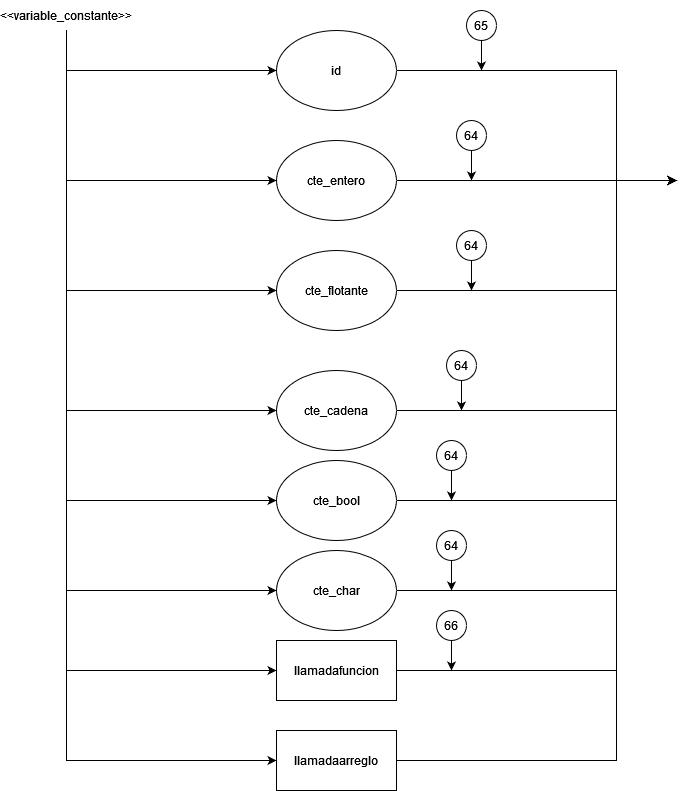
\includegraphics[width=\textwidth]{chapters/chapter3/figures/diagramas compis-variable_constante.drawio(1).png}
            \caption{Diagrama Variable\_Constante}
            \label{fig:my_label}
    \end{figure}
    \FloatBarrier
    \item Checar si la constante existe en la tabla de constantes, si no existe se agrega a la tabla de constantes con la dirección virtual apropiada. Agregar la dirección virtual de la constante a la pila de operandos
    \item Checar si el id existe en el scope local o global. Si existe agregar su dirección virtual a la pila de operandos.
    \item Checa si la llamada a función es de retorno. Si es de retorno crear una variable temporal con el valor actual de la variable global de la función y agregar el temporal a la pila de operandos
    
    
    \newpage
    
    %Llamada Arreglo
    \begin{figure}[!htbp]
            \centering
            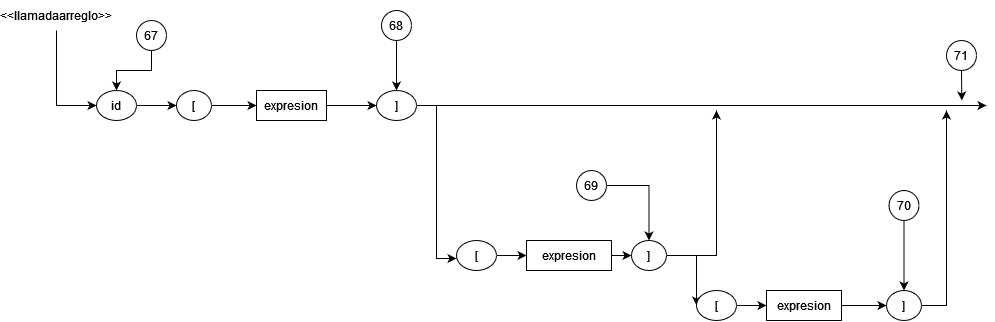
\includegraphics[width=\textwidth]{chapters/chapter3/figures/diagramas compis-llamadaarreglo.drawio.png}
            \caption{Diagrama Llamada Arreglo}
            \label{fig:my_label}
    \end{figure}
    \FloatBarrier
    \item Se revisa si el identificador es un arreglo. 
    \item Se hace pop a la pila de operandos y se revisa que el elemento recibido sea entero. Si es entero se agrega a la fila de subíndices.
    \item Se hace pop a la pila de operandos y se revisa que el elemento recibido sea entero. Si es entero se agrega a la fila de subíndices.
    \item Se hace pop a la pila de operandos y se revisa que el elemento recibido sea entero. Si es entero se agrega a la fila de subíndices.
    \item Se checa que la cantidad de subíndices leídos coincida con las dimensiones del arreglo, de ser así itera por los subíndices generando los cuádruplos de verificación y las sumas apropiadas para calcular la dirección virtual del arreglo accesado.
    
    \newpage
    % Llamada función
    \begin{figure}[!htbp]
            \centering
            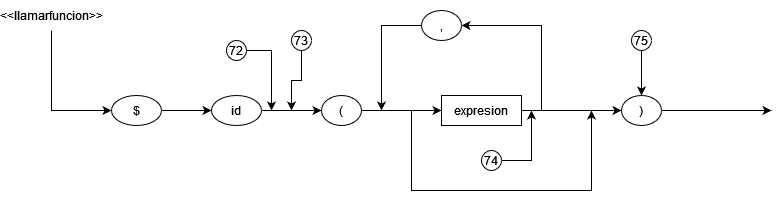
\includegraphics[width=\textwidth]{chapters/chapter3/figures/diagramas compis-llamarfuncion.drawio.png}
            \caption{Diagrama Llamada Función}
            \label{fig:my_label}
    \end{figure}
    \FloatBarrier
    
    \item Checar si es una función especial. Si es función especial, crear una variable global con el nombre y tipo de la función y la dirección de memoria apropiada.
    \item Obtener la información de los parámetros del directorio de funciones y generar el cuádruplo de era.
    \item Hacer pop a la pila de operandos y meter el elemento obtenido a una fila de parámetros.
    \item Comparar si los elementos de la fila de parámetros coinciden con los parámetros de la función. Si los elementos coinciden generar los cuádruplos de parameter apropiados para cada elemento de la fila.
    
    \newpage
    % Arreglo Textual
    \begin{figure}[!htbp]
            \centering
            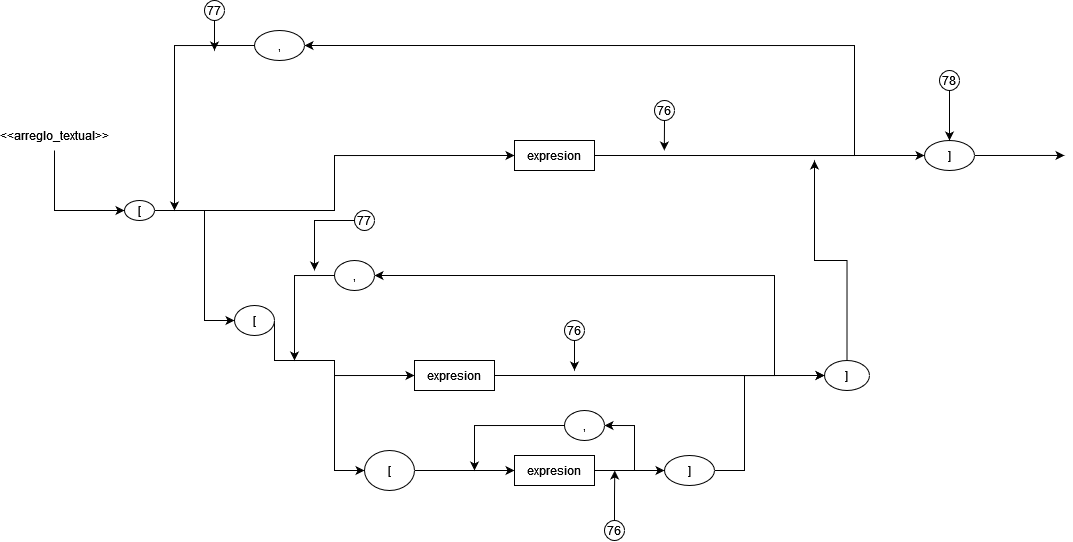
\includegraphics[width=\textwidth]{chapters/chapter3/figures/diagramas compis-arreglo_textual.drawio.png}
            \caption{Diagrama Arreglo\_Textual}
            \label{fig:my_label}
    \end{figure}
    \FloatBarrier
    
    \item Se checa el tipo de la expresión realizada y se mete a un stack auxiliar de tipos y se checa la congruencia de tipo con los demás leídos (si hay).
    \item Se checa la congruencia de la dimensión del elemento leído, si las dimensiones son diferentes se levanta un error. Igual se guarda el tamaño de las dimensiones leídas.
    \item Se calcula el tamaño del arreglo/cubo/matriz  
    
    

\end{enumerate}
\newpage
\FloatBarrier
%---------------------------------------------------------------------------------------
\section{Descripción de Administración de Memoria usado en la compilación}

Para la administración de memoria duarante compilación se usaron princiaplemente los siguientes elementos:

\begin{enumerate}

    \item Directorio de Funciones
    \item Vector de Cuadruplos y su contador
    \item Tabla de Constantes y su espejo
    \item Cubo Semantico
    \item Contadores Globales de Variables Globales y temporales
    \item Máximos de Variables y las direcciones de memoria
    \item Vector de relación linea código fuente a cuadruplo
    \item Variables auxiliares para el manejo de arreglos
    \item Pila de operadores, Pila de operandos y Pila de tipos
    \item Diccionario de funciones especiales
    
\end{enumerate}

Cada uno de estos se va a explicar con más detalle en las siguientes subsecciones.

\subsubsection{Directorio de Funciones y el Directorio de Funciones Especiales}

Para implementar el directorio de funciones se requería una estructura de datos que fuera de acceso rápido y que pudiera contener muchos tipos de variables e información dentro de ella. Afortunadamente en el lenguaje de Python no hay mucha restricción sobre el tipo de datos que se guardan en sus diferentes estructuras. Dado lo que se necesitaba que fuera el directorio de funciones se decidió utilizar la estructura de Diccionario de Python. Este nos permitiría guardar cualquier información necesaria con una llave única, además permite guardar cualquier otra estructura de datos dentro de cada entrada de un diccionario permitiendo una gran flexibilidad de la información que se puede guardar. También los diccionarios son de las estructuras son de rápido acceso para consultas.


\begin{table}[htbp]
    \centering
    %\tiny
    \begin{tabular}{|c|c|c|c|c|c|c|}
        nombre & tipo & address & params & varres & tmpres & vartab \\ \hline
        
         global & vacio & - & - & 1,0,1,1 & - & \tiny Dict de python de var  \\
         pop & vacio & -  & \tiny Dict de python de params & 1,0,3,1 & 14, 1, 2, 7, 0 & \tiny Dict de python de var \\
         principal & vacio & - & \tiny Dict de python de params & 1,0,1,1 & 14, 0, 0, 7, 0 & \tiny Dict de python de var  \\
    \end{tabular}
    \caption{Representación Lógica del directorio de funciones}
    \label{tab:my_label}
\end{table}
\FloatBarrier
Cada entrada de la tabla tiene cinco elementos importantes. El primero es el tipo de la función, este ayuda a identificar si la función tiene retorno o es vacía. La segunda es address. Esta es la dirección virtual de la función si es función de retorno. La tercera es params que es un diccionario de Python que tiene la información del tipo e información de arreglos si el parámetro es un arreglo. El tercero y cuarto elemento son una serie de contadores que representan los recursos locales y temporales respectivamente que tiene una función. El quinto elemento es la tabla de variables que contiene la información de las variables locales de la función.

En el caso de la entrada global, es la única entrada del directorio que no cuenta con información de variables temporales.


Para facilitar la integración de las funciones especiales en compilación también se usó una estructura muy similar al directorio de funciones. De esta manera se pueden usar muchos de los métodos para recorrer el directorio de funciones en el directorio de funciones especiales. Realmente la única diferencia que existe entre los dos es que el directorio de funciones especiales no cuenta con un contador de variables temporales ni una tabla de variables, ya que para ejecutar estas funciones en la máquina virtual solo se necesita saber la información de los parámetros.


\begin{table}[htbp]
    \centering
    %\tiny
    \begin{tabular}{|c|c|c|c|c|c|c|}
        nombre & tipo & address & params & varres \\ \hline
        
         normal & flotante & 1006 & \tiny Dict de python de params  & 2,0,0,0  \\
         modulo & flotante & 1007  & \tiny Dict de python de params & 2,0,0,0  \\
    \end{tabular}
    \caption{Representación Lógica del directorio de funciones especiales}
    \label{tab:my_label}
\end{table}
\FloatBarrier

\FloatBarrier
\subsubsection{Vector de Cuadruplos y su contador}

Para representar los cuádruplos se utilizaron la estructura de tuplas de Python. Pero un programa no cuenta con un solo cuádruplo sino una serie de múltiples cuádruplos ordenados que indican las instrucciones a ejecutar a la máquina virtual. Para lograr esto se creó una lista de tuplas, a la cual se le va agregando como en una fila cada cuádruplo generado. Para tener un mejor control sobre la cantidad de cuádruplos generados también se mantuvo una variable auxiliar global contadora de cuádruplos.

\begin{figure}[htbp]
    \centering
    \begin{lstlisting}[language=Python]
        ('GOTO','','',20)
    \end{lstlisting}
    \caption{Ejemplo de una tupla de Cuádruplo}
    \label{fig:my_label}
\end{figure}

\begin{figure}[htbp]
    \centering
    \begin{lstlisting}[language=Python]
        cuadruplos.append(('GOTOF',res,''))
        global sclines
        sclines.append(p.lineno(1))
        psaltos.append(cuadcount)
        cuadcount += 1
    \end{lstlisting}
    \caption{Ejemplo de generación de un cuádruplo}
    \label{fig:my_label}
\end{figure}
\FloatBarrier

\subsubsection{Tabla de Constantes y su espejo}

Como el directorio de funciones, la tabla de constantes también va a ser una estructura que va a ser consultada muy frecuente mente. Como se había mencionado previamente, el diccionario de Python también es una buena solución para poder guardar y acceder con mucha facilidad información de manera frecuente. Por ello se optó por usar también el diccionario de Python para representar la tabla de constantes.


\begin{table}[htbp]
    \centering
    \begin{tabular}{c|c}
         Constante & Dirección \\ \hline
         25000 & 2 \\
         25001 & 1 \\
         310000 & "Hola" \\
    \end{tabular}
    \caption{Representación Lógica de la tabla de constantes}
    \label{tab:my_label}
\end{table}
\FloatBarrier

\begin{figure}[htbp]
    \centering
    \begin{lstlisting}[language=Python]
        {                                         
            "2": 25000,                            
            "1": 25001,                            
            "3": 25002,                            
            "1001": 25003,                         
            "1003": 25004,                         
            "3000": 25005,                         
            "0": 25006,                            
            "5": 25007,                            
            "\"Factorial de n \\n\"": 31000,       
            "10": 25008,                           
            "\"Factorial Secuencial : \"": 31001,  
            "\"------\\n hola aka =\"": 31002      
        }                                           
    \end{lstlisting}
    \caption{Ejemplo de el diccionario de constantes}
    \label{fig:my_label}
\end{figure}
\FloatBarrier

Como Python no es un lenguaje fuertemente tipado, para generar las llaves del diccionario se transforma a string la constante para poderla encontrar fácilmente. También para reducir el tiempo de ejecución a la hora de crear el archivo obj, se mantiene una copia de la tabla de constantes con el formato correcto para la máquina virtual.
\begin{figure}[htbp]
    \centering
    \begin{lstlisting}[language=Python]
        {
            "25000": 3,
            "25001": 1,
            "25002": 9,
            "25003": 9003,
            "25004": 14001,
            "25005": 9006,
            "25006": 10,
            "25007": 30,
            "25008": 2,
            "25009": 1000000,
            "25010": 20,
            "30000": true,
            "31000": "\"Hola Mundo\"",
            "25011": 0,
            "31002": "\"Iteracion por la matriz\"",
            "31003": "\"Iteracion por el cubo\"",
            "31004": "\"\\t--Dim2\"",
            "31005": "\"\\t\\t---Dim 3\"",
            "31006": "\"Probando arreglos textuales\"",
            "29000": "'a'",
            "25012": 4,
            "25013": 5,
            "25014": 6,
            "29001": "'b'",
            "29002": "'c'",
            "30001": false,
            "25015": 127
        }
    \end{lstlisting}
    \caption{Ejemplo de el diccionario de constantes para la máquina virtual}
    \label{fig:my_label}
\end{figure}

\FloatBarrier

\subsection{Tabla de variables}

Para la tabla de variables también se necesitó una estructura de datos que se rápida de acceder y modificar. Como se mencionó con el directorio de funciones, el diccionario de Python resulto ser una estructura de datos que se adaptaba muy bien a solucionar este problema. Por ello también se utilizó un diccionario de Python para representar la tabla de variables.


\begin{table}[htbp]
    \centering
    \begin{tabular}{c|c|c|c|c}
        nombre & tipo & dirección & dims & dimlen   \\
        a & entero & 1000 & - & - \\
        b & entero & 1001 & 2 & [3,4], [4,0] \\
    \end{tabular}
    \caption{Representación Lógica de la tabla de variables}
    \label{tab:my_label}
\end{table}
\FloatBarrier
El diccionario de la tabla de variables constaba de que cada llave fuera el nombre de la variable y que dentro de esa llave se guardara otro diccionario con la información de la variable. Este diccionario tiene lo que es el tipo de la variable, su dirección de memoria, y si es un arreglo, las dimensiones del arreglo y la información para calcular la indexación.

\subsubsection{Cubo Semántico}

Para el cubo semántico se decidió ir por una estructura que pudiera ser accesada rápidamente y que pudiera dar el resultado de una operación con llaves sencillas. Ya que se trabajó en el lenguaje de Python, se aprovechó de la estructura nativa de diccionarios. Estos pueden ser accesados rápidamente y se le pueden asignar llaves a cada entrada. Para hacer el código legible se decidió estructurar el cubo como un diccionario de diccionarios. De esta manera la llamada al cubo semántico sería accesando al cubo con la primera llave siendo el operador, y las otras dos llaves siendo el operando izquierdo y el operando derecho.


\begin{table}
    \centering
    \caption{Tabla representando el cubo semántico}
    \small
    \begin{tabular}{||c c || c c c c c c c c c c c c c||} 
         
         OpIzq & OpDer & $=$ & $\parallel$ & \&\& & \textless & \textgreater & \textless $=$ & \textgreater $=$ & !$=$ & $==$ & $+$ & $-$ & * & \textbackslash \\ [0.5ex] 
         \hline\hline
         ent & ent & ent & bool & bool & bool & bool & bool & bool & bool & bool & ent & ent & ent & ent \\ 
         \hline
         ent & flot & ent & bool & bool & bool & bool & bool & bool & bool & bool & flot & flot & flot & flot \\ 
         \hline
         ent & char & ent & bool & bool & bool & bool & bool & bool & bool & bool & ent & ent & ent & ent \\ 
         \hline
         ent & bool & ent & bool & bool & bool & bool & bool & bool & bool & bool & ent & ent & ent & ent \\ 
         \hline
         ent & cadena & err & err & err & err & err & err & err & err & err & err & err & err & err \\ 
         \hline
         flot & ent & flot & bool & bool & bool & bool & bool & bool & bool & bool & flot & flot & flot & flot \\ 
         \hline
         flot & flot & flot & bool & bool & bool & bool & bool & bool & bool & bool & flot & flot & flot & flot \\ 
         \hline
         flot & char & flot & bool & bool & bool & bool & bool & bool & bool & bool & flot & flot & flot & flot \\ 
         \hline
         flot & bool & flot & bool & bool & bool & bool & bool & bool & bool & bool & flot & flot & flot & flot \\ 
         \hline
         flot & cadena & err & err & err & err & err & err & err & err & err & err & err & err & err \\ 
         \hline
         char & ent & char & bool & bool & bool & bool & bool & bool & bool & bool & ent & ent & ent & ent \\ 
         \hline
         char & flot & char & bool & bool & bool & bool & bool & bool & bool & bool & flot & flot & flot & flot \\ 
         \hline
         char & char & char & bool & bool & bool & bool & bool & bool & bool & bool & ent & ent & ent & ent \\ 
         \hline
         char & bool & char & bool & bool & bool & bool & bool & bool & bool & bool & ent & ent & ent & ent \\ 
         \hline
         char & cadena & err & err & err & err & err & err & err & err & err & err & err & err & err \\ 
         \hline
         bool & ent & bool & bool & bool & bool & bool & bool & bool & bool & bool & ent & ent & ent & ent \\ 
         \hline
         bool & flot & bool & bool & bool & bool & bool & bool & bool & bool & bool & flot & flot & flot & flot \\ 
         \hline
         bool & char & bool & bool & bool & bool & bool & bool & bool & bool & bool & ent & ent & ent & ent \\ 
         \hline
         bool & bool & bool & bool & bool & bool & bool & bool & bool & bool & bool & ent & ent & ent & ent \\ 
         \hline
         bool & cadena & err & err & err & err & err & err & err & err & err & err & err & err & err \\ 
         \hline
         cadena & ent & err & err & err & err & err & err & err & err & err & err & err & err & err \\ 
         \hline
         cadena & flot & err & err & err & err & err & err & err & err & err & err & err & err & err \\ 
         \hline
         cadena & char & err & err & err & err & err & err & err & err & err & err & err & err & err \\ 
         \hline
         cadena & bool & err & err & err & err & err & err & err & err & err & err & err & err & err \\ 
         \hline
         cadena & err & err & err & err & err & err & err & err & err & err & err & err & err & err \\ 
        
         
        
        \end{tabular}
        \begin{itemize}
            \item ent : Entero
            \item flot : Flotante
            \item err : Error
        \end{itemize}
    
\end{table}
\FloatBarrier

\begin{figure}[htbp]
    \centering
    \begin{lstlisting}[language=Python]
        rettype = ptipo.pop()
        if (cubosem['='][functipo][rettype] != 'error'):
            dprint('Cubo dice: ',cubosem['='][functipo][rettype])
            retop = pilaoperand.pop()
            ......
    \end{lstlisting}
    \caption{Ejemplo del uso de el Cubo Semántico}
    \label{fig:my_label}
\end{figure}
\FloatBarrier
\begin{figure}[htbp]
    \centering
    \begin{lstlisting}[language=Python]
        cubosem = {
        '=':{
            'entero':{
                        'entero':'entero',
                        'flotante': 'entero',
                        'char':'entero',
                        'bool': 'entero',
                        'cadena':'error'
                    },
            'flotante':{
                        'entero':'flotante',
                        'flotante': 'flotante',
                        'char':'flotante',
                        'bool': 'flotante',
                        'cadena':'error'
                    },
            'char':{
                        'entero':'char',
                        'flotante': 'char',
                        'char':'char',
                        'bool': 'char',
                        'cadena':'error'
                    },
            'bool':{
                        'entero':'bool',
                        'flotante': 'bool',
                        'char':'bool',
                        'bool': 'bool',
                        'cadena':'error'
                    },
            'cadena':{
                        'entero':'error',
                        'flotante': 'error',
                        'char':'error',
                        'bool': 'error',
                        'cadena':'err'
                    },

            },
        .....
    \end{lstlisting}
    \caption{Muestra de la primera entrada del cubo semántico}
    \label{fig:my_label}
\end{figure}
\FloatBarrier




\subsubsection{Contadores Globales de Variables Globales y temporales, Máximos de Variables y las Direcciones de Memoria}

Para mantener un registro del uso de recursos dentro del programa durante el proceso de compilación se crearon variables globales que funcionaban como contadores sobre cada tipo de variable. Cada vez que se generaba una nueva variable se aumentaba el contador y se verificaba que no se pasara de los máximos del tipo permitidos. Estos contadores se dejaron como variables globales porque había múltiples acciones semánticas que requerían consultar o actualizar sus valores. Para mantener legibilidad y por simplicidad se optó por dejarlo como variables globales.

\begin{table}[htbp]
    \centering
    \begin{tabular}{c|c|c|c|c}
        \multicolumn{5}{c}{Globales} \\\hline
         Enteros & Flotantes & Caracteres & Booleanos & Apuntadores  \\
          1 & 2 & 0 & 3 & 0 \\\hline\hline
          
          \multicolumn{5}{c}{Temporales} \\
         Enteros & Flotantes & Caracteres & Booleanos & Apuntadores  \\
          8 & 2 & 0 & 6 & 0 
    \end{tabular}
    \caption{Representación Lógica de los Contadores Globales}
    \label{tab:my_label}
\end{table}
\FloatBarrier
Similar que con los contadores globales también se dejó los máximos de variables y de direcciones de memoria como variables globales para mantener legibilidad y simplicidad en el código. Como muchas de las acciones semánticas también interactuar con ellas se mantienen globales.

\subsubsection{Vector de relación línea código fuente a cuádruplo}

Para desarrollar mensajes de error más detallados en la máquina virtual, se necesitaba saber en qué línea de código se causó el error. Para resolver este problema se creó una lista que aprovecha el rastreador de tokens del lexer de \emph{ply} para guardar el número de la línea del código fuente en relación con un cuádruplo. Esta lista va creciendo a la par que la lista de cuádruplos y es pasada como información a la máquina virtual para que pueda usarla en sus mensajes de error.


\begin{figure}[htbp]
    \centering
    \begin{lstlisting}
    // La lista de cuadruplos
        Cuadruplos = [('GOTO','MAIN','',''), 
        ("*", 25006, 25007, 17000), 
        ("/", 17000, 25007, 17001), 
        ("*", 17001, 25008, 17002), 
        ......]
    // Lista de la linea de codigo fuente que la creo
        sclines = [1, 9, 9, 9, 9, ......]
    \end{lstlisting}
    \caption{Ejemplo de como se ve la relación de cuádruplos contra líneas de código fuente}
    \label{fig:my_label}
\end{figure}
\FloatBarrier
\subsubsection{Variables auxiliares para el manejo de arreglos}

Para el cálculo de la información de la indexación de arreglos se optó por dejar las variables como variables globales. Como no son muchas las variables para el cálculo de la fórmula de indexación, ya que este lenguaje se limita hasta cubos nada más, no se vio necesario crear una estructura extra para manejar su información. De igual manera, como son múltiples acciones semánticas que utilizan estas variables por conveniencia se dejaron como variables globales.


\begin{table}[htbp]
    \centering
    \begin{tabular}{|c|c|}
       R  &  1\\
      at1 & 2 \\
      at2 & 3 \\
      at3 & 0 \\
    \end{tabular}
    \caption{Representación Lógica de las Varables Auxiliares de arreglos}
    \label{tab:my_label}
\end{table}

\FloatBarrier
\subsubsection{Pila de operadores, Pila de operandos y Pila de tipos}

Para el manejo de la lógica de expresiones como visto en clase se necesitaba utilizar una estructura stack para el manejo de las acciones semánticas. Python no cuenta con una estructura stack, pero cuenta con métodos que simulan a un stack en su estructura de lista. Por ello se manejó la Pila de Operadores, Pila de Operandos y la Pila de tipos como listas las cuales solo se podían interactuar con usando los métodos de \emph{pop} y \emph{append} que tienen las listas.

\begin{table}[htbp]
    \centering
    \begin{tabular}{c|c c c c}
         \hline
        Pila de Operadores & + & * & & ....   \\\hline \hline
        Pila de Operandos &  A & 1000 & x\_inicial & ....\\\hline \hline
        Pila de Tipos & entero & entero & entero & .... \\\hline \hline
    \end{tabular}
    \caption{Representación Lógica de las Pilas}
    \label{tab:my_label}
\end{table}
